\subsection{Function discriminant analysis, FDA}

 
\begin{figure}[h]
 \begin{minipage}{8.5cm}
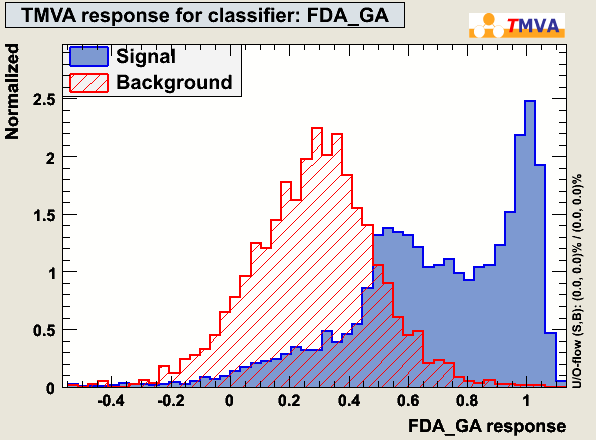
\includegraphics[width=1.0\textwidth]{images/pkMva_FDA_GA.png}
\end{minipage}
 \hfill
\begin{minipage}{8.5cm}
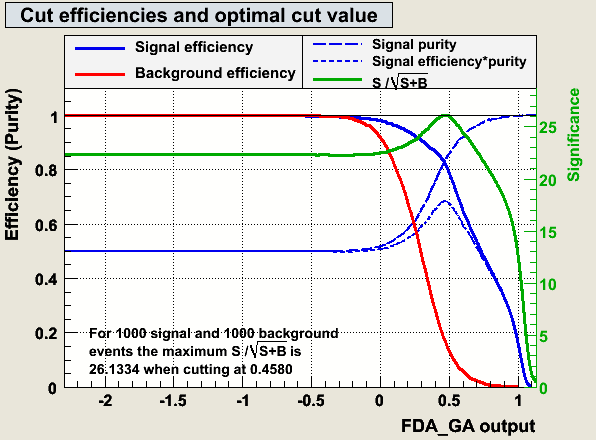
\includegraphics[width=1.0\textwidth]{images/pkMvaEffs_FDA_GA.png}
\end{minipage}
\caption{Left: mvaFDA using genetic algorighm (GA). Right: FDA GA}
\label{fig:pkMvaFDAGA}
%\label{fig:pkMvaEffsFDAGA}
\end{figure}


\begin{figure}[h]
 \begin{minipage}{8.5cm}
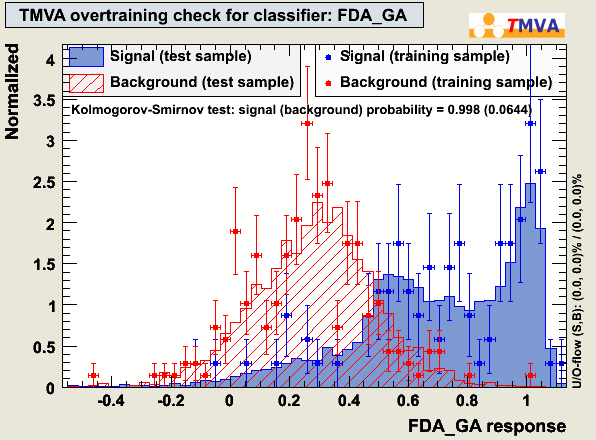
\includegraphics[width=1.0\textwidth]{images/pkOvertrain_FDA_GA.png}
\end{minipage}
 \hfill
\begin{minipage}{8.5cm}
FDA GA
\end{minipage}

\label{fig:pkOvertrainFDAGA}
\end{figure}


\subsection{k-nearest neighbour method, kNN}

 
\begin{figure}[h]
 \begin{minipage}{8.5cm}
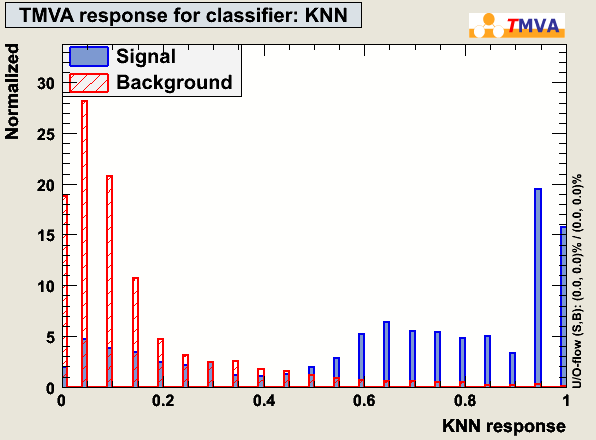
\includegraphics[width=1.0\textwidth]{images/pkMva_KNN.png}
\end{minipage}
 \hfill
\begin{minipage}{8.5cm}
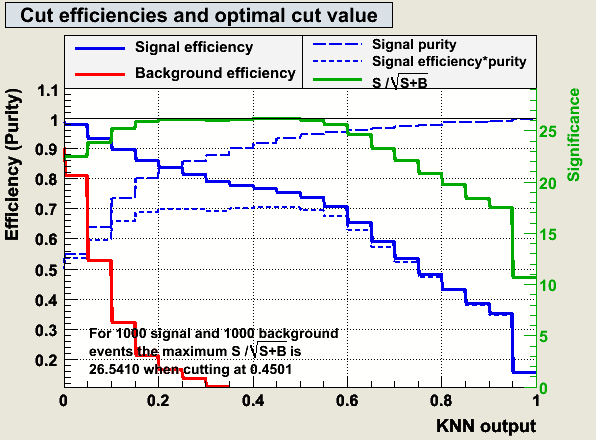
\includegraphics[width=1.0\textwidth]{images/pkMvaEffs_KNN.png}
\end{minipage}
\caption{Left: MVAKNN. Right: KNN effs}
\label{fig:pkMvaKNN}
%\label{fig:pkMvaEffsKNN}
\end{figure}


\begin{figure}[h]
 \begin{minipage}{8.5cm}
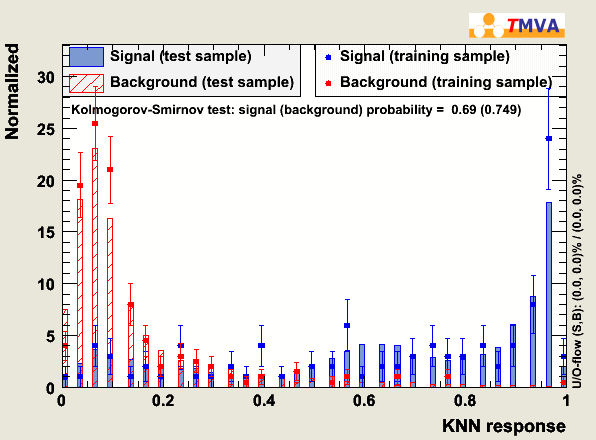
\includegraphics[width=1.0\textwidth]{images/pkOvertrain_KNN.png}
\end{minipage}
 \hfill
\begin{minipage}{8.5cm}
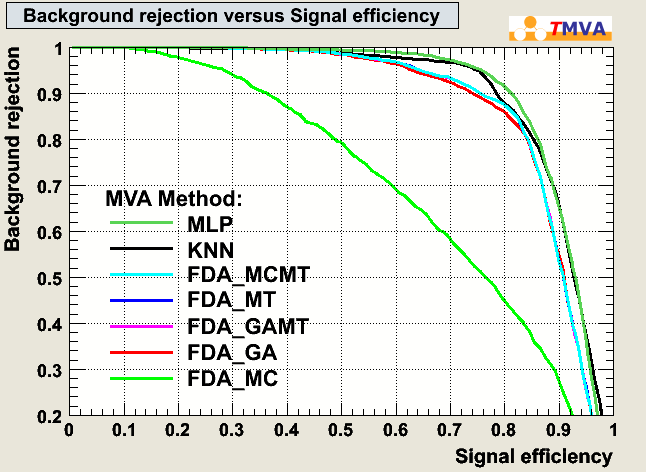
\includegraphics[width=1.0\textwidth]{images/pkRejBvsS.png}
\end{minipage}
\caption{Left: KNN. Right: ROC curve (MLP added as a benchmark)}
\label{fig:pkOvertrainKNN}
%\label{fig:pkRejBvsS}
\end{figure}

\clearpage
